\documentclass[convert, tikz, border=5pt]{standalone}
\usetikzlibrary{positioning, calc}

\begin{document}

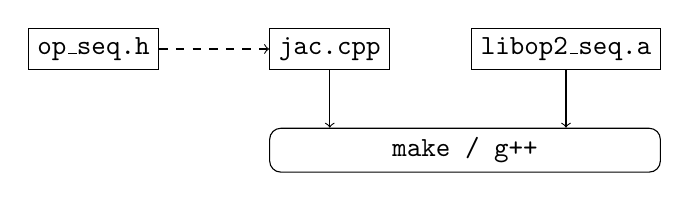
\begin{tikzpicture}[every node/.style={draw, font=\tt}, node distance=3cm, align=center]
    \node (opseq)     []               {op\_seq.h};
    \node (jac)       [right of=opseq] {jac.cpp};
    \node (libraries) [right of=jac]   {libop2\_seq.a};

    \path let
        \p1=(jac.west),
        \p2=(libraries.east)
    in node (build) [
        rounded corners,
        below=1cm of jac.west, anchor=north west, minimum width=\x2-\x1-\pgflinewidth
    ] {make / g++};

    \draw[dashed, ->] (opseq)     -- (jac);

    \draw[->]         (jac)       -- (jac       |- build.north);
    \draw[->]         (libraries) -- (libraries |- build.north);
\end{tikzpicture}

\end{document}
